% =============================================================================
% OVERLEAF — copy/paste instructions
% -----------------------------------------------------------------------------
% 1. New Project → Blank Project → paste this file as main.tex
% 2. New Folder → figures/  and upload:
%      figure1_overview.png
%      figure2_evaluation.png
%      figure3_qualitative.png
% 3. Compiler → pdfLaTeX → Recompile → Download PDF
% =============================================================================

\documentclass[10pt,twocolumn,letterpaper]{article}

\usepackage[margin=0.75in]{geometry}
\usepackage{graphicx}
\graphicspath{{figures/}}
\usepackage{booktabs}
\usepackage{amsmath}
\usepackage{caption}
\usepackage{hyperref}
\usepackage{enumitem}

\hypersetup{colorlinks=true,urlcolor=blue!60!black,linkcolor=black}
\captionsetup{font=small,labelfont=bf,skip=4pt}
\setlist{nosep,leftmargin=*}

\title{\Large\textbf{SpatialLens Assist: Motion-Aware Hazard Detection\\for Campus Navigation}}

\author{%
  \textbf{Diego Sanchez} \\
  Department of Computer Science \\
  Stanford University \\
  \texttt{dsanh14@stanford.edu}
}

\date{}

\begin{document}

\maketitle
\vspace{-0.8em}
\begin{center}
\small
CS131 Final Project \quad|\quad May 2026 \quad|\quad
\href{https://github.com/dsanh14/SpatialLens}{github.com/dsanh14/SpatialLens}
\end{center}
\vspace{0.4em}

\begin{abstract}
Assistive navigation systems must communicate not only \emph{what} is nearby but \emph{how} it moves relative to the walker. We present \textbf{SpatialLens Assist}, an offline pipeline that converts short campus-walkway videos into motion-aware hazard alerts for blind and low-vision pedestrians. Each tracked object is classified into one of six hazard categories using a rule cascade over ego-motion-compensated optical flow and bounding-box growth, with a textual evidence string for every prediction. On 11 campus videos and 61 manually labeled tracks, the system achieves \textbf{93.3\,\% decidable accuracy} on tracks with $\ge$3 frames and \textbf{82.5\,\% overall accuracy}; the gap is dominated by deliberate \texttt{short\_track} abstentions on 1--2 frame tracker fragments. The safety-critical \texttt{approaching} class reaches precision 0.95 and recall 0.88. Ablations show that raising the tracker frame-gap buffer (+15.3\,pp) and a v2 rule cascade (+3.6\,pp vs.\ removing \texttt{strong\_crossing}) are the largest accuracy drivers; an opt-in ByteTrack backend is a negative result for low-fps offline footage.
\end{abstract}

\section{Introduction}

Camera-based assistive navigation has progressed rapidly through object detectors that can localize pedestrians, bicycles, and other road users in real time. For a blind pedestrian, however, knowing that a bicycle is present in the frame is insufficient: the relevant question is whether it is \emph{approaching}, \emph{crossing the path}, or \emph{moving away}. Single-frame appearance cues are ambiguous---a distant cyclist and a parked bicycle can look similar---while motion over time disambiguates intent.

SpatialLens Assist targets this gap with a lightweight, explainable pipeline that runs on iPhone campus footage sampled at 2\,fps. The system detects objects, tracks them across frames, extracts motion features with ego-motion compensation, classifies each track into a hazard label, and emits natural-language alerts that quote the classifier's evidence string.

\subsection{Problem Statement}

Given a short egocentric video from a handheld phone, produce for each persistent object track:
(1)~a hazard label from
\{\texttt{approaching}, \texttt{crossing\_left\_to\_right}, \texttt{crossing\_right\_to\_left}, \texttt{moving\_away}, \texttt{static}, \texttt{uncertain}\};
(2)~a confidence tier; and
(3)~a human-readable alert suitable for text-to-speech output.
The system must abstain honestly when motion evidence is insufficient rather than guess.

\subsection{Contributions}

This report documents a complete week-1--3 pipeline with:
(i)~ego-motion-compensated motion features for hand-held footage;
(ii)~a priority-ordered rule cascade with explainable \texttt{uncertain\_reason} sub-labels;
(iii)~a 61-track manually labeled evaluation set across 11 campus videos;
(iv)~ablation studies on tracker frame-gap, classifier cascade design, and ByteTrack; and
(v)~reproducible scripts, 80 unit tests, and slide-ready demo assets.

\section{Related Work}

Object detection for assistive navigation commonly builds on YOLO-family detectors~\cite{yolo} applied to egocentric video. Multi-object tracking for offline clips often uses IoU matching or Kalman-filter trackers such as ByteTrack~\cite{bytetrack}; the latter is designed for high-fps real-time streams and may discard low-confidence detections that are common at 2\,fps sampling. Motion analysis for collision warning traditionally combines optical flow~\cite{farneback} with heuristics on bounding-box scale change and image-plane displacement. Learned trajectory classifiers require labeled training data that was unavailable at project start; we therefore adopt an interpretable rule cascade whose thresholds can be tuned against a small hand-labeled set without overfitting.

\section{Methods}

Figure~\ref{fig:overview} summarizes the end-to-end architecture. The pipeline has five stages: detection, tracking, motion-feature extraction, hazard classification, and alert generation.

\subsection{Detection and Tracking}

\textbf{Detection.} Ultralytics YOLOv8n~\cite{yolo} on COCO classes \{person, bicycle, motorcycle, skateboard\} with confidence threshold $\tau=0.35$. Scooters are not a native COCO class and may appear as \texttt{skateboard}.

\textbf{Tracking.} A per-class IoU+centroid matcher links detections across frames using score $0.7\cdot\text{IoU} + 0.3(1-\hat d)$, where $\hat d$ is normalized centroid distance. Unmatched detections spawn new track IDs; unmatched tracks are kept for up to \texttt{max\_frame\_gap=4} frames before deletion. An opt-in ByteTrack backend was implemented but not adopted (Section~\ref{sec:ablations}).

\subsection{Motion Feature Extraction}

For each track we compute:
\textbf{(i)} start-to-end centroid displacement $(dx, dy)$ and normalized horizontal displacement $dx\_\text{norm}$;
\textbf{(ii)} bounding-box growth ratio $\text{growth}=(A_\text{end}-A_\text{start})/A_\text{start}$;
\textbf{(iii)} median Farneback optical-flow magnitude and direction inside the bbox; and
\textbf{(iv)} frame-differencing overlap within the bbox.

Both flow and frame-diff are \emph{ego-motion compensated}: the global median flow vector is subtracted from per-object flow, and consecutive frames are aligned with ECC (translation model) before differencing. This reduces false motion from hand-held camera pans.

\subsection{Hazard Rule Cascade}

The classifier applies a fixed priority cascade. Tracks with fewer than \texttt{min\_track\_frames=3} abstain as \texttt{uncertain/short\_track}. Otherwise rules fire in order:
\textbf{(1)}~\texttt{moving\_away} if $\text{growth} < -0.15$;
\textbf{(2)}~\texttt{strong\_crossing} if $|dx\_\text{norm}| > 0.50$ (v2 addition);
\textbf{(3)}~\texttt{crossing\_*} if $|dx\_\text{norm}| > 0.12$ and growth is below threshold;
\textbf{(4)}~\texttt{approaching} if growth and \texttt{approach\_score} exceed thresholds;
\textbf{(5)}~\texttt{static} if displacement and flow are near zero; else
\textbf{(6)}~\texttt{uncertain} with a reason tag (\texttt{near\_approaching}, \texttt{low\_signal}, etc.).
Every label includes a textual evidence string used by the alert layer.

\subsection{Assistive Alerts and Explainability}

The alert module maps hazard labels to spoken messages (e.g.\ ``Bike approaching from the left.''). For \texttt{uncertain} tracks the message quotes the \texttt{uncertain\_reason}: ``Person detected briefly; not enough frames to judge motion'' for \texttt{short\_track}. Annotated frames and MP4 demos overlay bbox color, hazard label, and evidence text; videos are encoded with H.264 for macOS QuickTime compatibility.

\begin{figure*}[t]
\centering
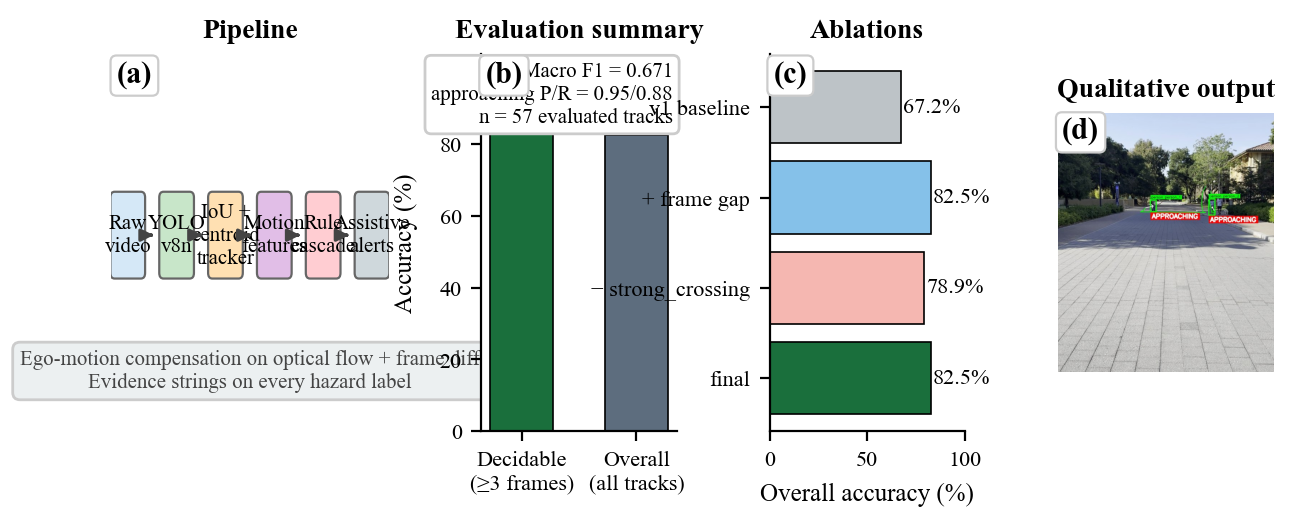
\includegraphics[width=\textwidth]{figure1_overview.png}
\caption{Overview of SpatialLens Assist.
(\textbf{a})~End-to-end pipeline.
(\textbf{b})~Decidable vs.\ overall accuracy on 57 matched tracks.
(\textbf{c})~Ablation accuracies.
(\textbf{d})~Qualitative hazard overlay from IMG\_4976.}
\label{fig:overview}
\end{figure*}

\section{Dataset and Evaluation Protocol}

\textbf{Videos.} Eleven \emph{controlled} campus-walk clips (IMG\_4972--4982) filmed on Stanford walkways at 2\,fps; two additional \emph{uncontrolled} natural-walk clips (IMG\_4989--4990) for qualitative demo only.

\textbf{Labels.} Ground truth in \texttt{data/labels/hazard\_labels.csv}: 61 tracks manually labeled with hazard category and reviewer notes. Four labeled tracks were merged by the tracker and appear as 57 evaluated prediction--label pairs.

\textbf{Metrics.} For matched tracks we report:
\begin{enumerate}[label=(\roman*),leftmargin=*]
\item \textbf{Overall accuracy:} fraction of tracks where predicted label equals ground truth.
\item \textbf{Decidable accuracy:} same, restricted to tracks with $\ge$3 frames---the regime the motion classifier is designed for.
\item \textbf{Per-class precision, recall, F1} and macro-F1.
\item \textbf{Confusion matrix} (rows = true, columns = predicted).
\end{enumerate}

\section{Results}

\subsection{Quantitative Results}
\label{sec:quant}

Table~\ref{tab:perclass} reports per-class metrics on the aggregate labeled set. Table~\ref{tab:ablation} summarizes ablations. Headline numbers: \textbf{93.3\,\% decidable} (28/30), \textbf{82.5\,\% overall} (47/57), macro-F1 0.671. The safety-critical \texttt{approaching} class---the primary collision-warning category---achieves F1 0.91 at precision 0.95.

\begin{table}[h]
\centering
\caption{Per-class metrics on 57 evaluated tracks (11 videos).}
\label{tab:perclass}
\small
\begin{tabular}{@{}lrrrr@{}}
\toprule
Class & Prec. & Rec. & F1 & $n$ \\
\midrule
approaching & 0.95 & 0.88 & 0.91 & 24 \\
moving\_away & 1.00 & 0.78 & 0.88 & 9 \\
crossing\_R$\to$L & 1.00 & 0.67 & 0.80 & 3 \\
uncertain & 0.63 & 1.00 & 0.77 & 15 \\
crossing\_L$\to$R & 1.00 & 0.50 & 0.67 & 4 \\
static & 0.00 & 0.00 & 0.00 & 2 \\
\midrule
Macro F1 & \multicolumn{4}{c}{0.671} \\
Decidable acc.\ ($\ge$3 fr.) & \multicolumn{4}{c}{93.3\,\% (28/30)} \\
Overall accuracy & \multicolumn{4}{c}{82.5\,\% (47/57)} \\
\bottomrule
\end{tabular}
\end{table}

\begin{table}[h]
\centering
\caption{Ablation study on the labeled evaluation set.}
\label{tab:ablation}
\small
\begin{tabular}{@{}lc@{}}
\toprule
Configuration & Accuracy \\
\midrule
v1 baseline (\texttt{max\_frame\_gap=2}) & 67.2\,\% \\
+ frame gap ($2\to4$) & 82.5\,\% \\
$-$ \texttt{strong\_crossing} rule (v2 cascade) & 78.9\,\% \\
Final (v2 cascade + gap=4) & 82.5\,\% \\
ByteTrack backend (tuned, low fps) & $\sim$50\,\% det.\ retained \\
\bottomrule
\end{tabular}
\end{table}

\subsection{Failure Analysis}

Figure~\ref{fig:eval} decomposes remaining errors.
\textbf{Confusion matrix (a):} the \texttt{approaching} column is clean; most off-diagonal mass flows to \texttt{uncertain} on 1--2 frame tracker fragments.
\textbf{Uncertain reasons (b):} \texttt{short\_track} accounts for 98\,\% of uncertain predictions (39/40), indicating tracker fragmentation rather than classifier confusion as the dominant failure mode.
\textbf{Priority conflicts} (diagonal walkers labeled \texttt{approaching} instead of \texttt{crossing}) were reduced by the v2 cascade; one \texttt{moving\_away} track is still misclassified as \texttt{approaching} when bbox growth briefly spikes.
\textbf{Static objects} (parked bicycles) appear for only one frame and correctly abstain as \texttt{short\_track}, yielding 0\,\% static F1 on the labeled set.

\begin{figure*}[t]
\centering
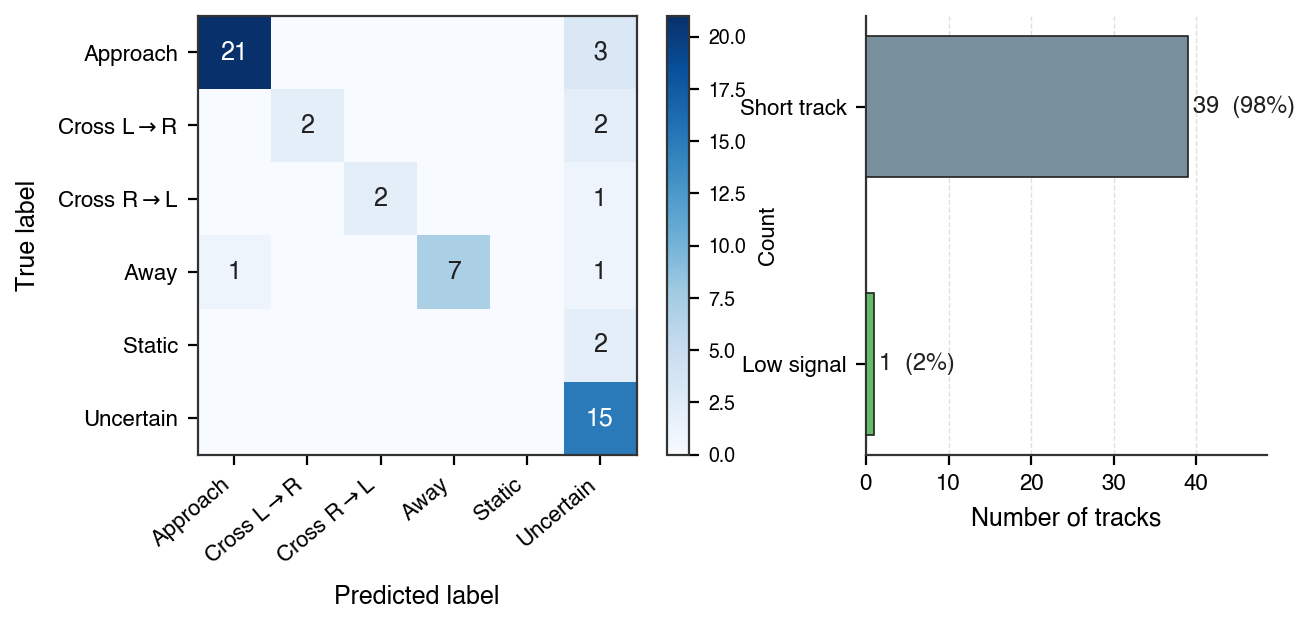
\includegraphics[width=\textwidth]{figure2_evaluation.png}
\caption{Evaluation and failure analysis.
(\textbf{a})~Aggregate confusion matrix.
(\textbf{b})~\texttt{uncertain\_reason} breakdown; \texttt{short\_track} dominates, motivating post-hoc track merging.}
\label{fig:eval}
\end{figure*}

\subsection{Qualitative Results}

Figure~\ref{fig:qual} shows representative outputs. Trajectories from IMG\_4974 illustrate centroid paths used for crossing detection. The hazard overlay from IMG\_4976 highlights approaching pedestrians with red \texttt{APPROACHING} banners and prints evidence strings below each bbox. Uncontrolled clip IMG\_4989 exposes the remaining limit: $\sim$50\,\% of tracks fall to \texttt{uncertain/short\_track} when objects pass through the frame in only 1--2 sampled frames.

\begin{figure*}[t]
\centering
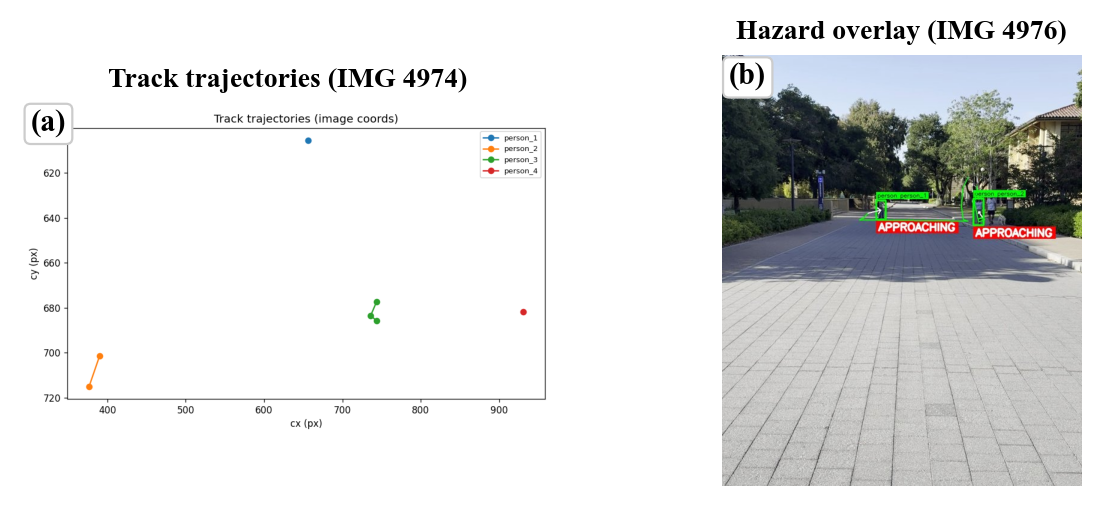
\includegraphics[width=\textwidth]{figure3_qualitative.png}
\caption{Qualitative pipeline outputs.
(\textbf{a})~Track trajectories in image coordinates (IMG\_4974).
(\textbf{b})~Hazard-annotated frame with evidence strings (IMG\_4976).}
\label{fig:qual}
\end{figure*}

\section{Discussion and Deviations}
\label{sec:ablations}

\textbf{Rule cascade vs.\ learned classifier.} The proposal hedged between learned and rule-based classification. We committed to rules because no labeled set existed in week~1, rules produce explicit evidence strings, and thresholds tune against 61 labels without overfitting a deep model.

\textbf{Ego-motion compensation.} Added in week~3 after hand-held pans produced false-positive flow; median-flow subtraction + ECC alignment reduced spurious \texttt{approaching} labels.

\textbf{ByteTrack (negative result).} Implemented and benchmarked as a drop-in tracker replacement. Even tuned for 2\,fps offline data, ByteTrack dropped roughly half the detections---its Kalman design assumes high-fps real-time streams. The simpler IoU+centroid matcher remains default.

\textbf{Scope unchanged.} Hazard taxonomy, campus-walkway setting, and assistive-alert framing match the proposal.

\section{Remaining Work}

With one week remaining: \textbf{(day~1)} optional post-hoc track merger (greedy per-class merge of fragments $\le$3 frames apart, target 87--90\,\% overall); \textbf{(days~2--4)} lock numbers, methods chapter, failure analysis; \textbf{(days~5--6)} slide deck from \texttt{outputs/slide\_assets/}; \textbf{(day~7)} buffer. Stretch goals (YOLOv8s on IMG\_4977, slow-approach softening rule) are off the critical path; we will not re-sample or re-label, as that would invalidate the evaluation set. All code and configs are versioned; the pipeline runs end-to-end via \texttt{python scripts/run\_final\_pipeline.py --all}.

\section{Conclusion}

SpatialLens Assist demonstrates that motion-aware hazard classification for campus navigation is feasible with a lightweight, explainable pipeline. On tracks with sufficient temporal support, decidable accuracy reaches 93.3\,\%; the remaining overall gap is largely tracker fragmentation, not classifier error. The v2 rule cascade and frame-gap tuning provide the largest gains; ByteTrack is a useful negative result for low-fps offline settings. Post-hoc track merging is the most promising next step before the final report and demo.

\begin{thebibliography}{9}
\bibitem{yolo}
J.~Redmon and A.~Farhadi.
YOLOv3: An incremental improvement.
\emph{arXiv:1804.02767}, 2018.
Ultralytics YOLOv8 used in implementation.

\bibitem{bytetrack}
Y.~Zhang et al.
ByteTrack: Multi-object tracking by associating every detection box.
\emph{ECCV}, 2022.

\bibitem{farneback}
G.~Farneb{\"a}ck.
Two-frame motion estimation based on polynomial expansion.
\emph{SCIA}, 2003.

\bibitem{ecc}
G.~Evangelidis and E.~Psarakis.
Parametric image alignment using enhanced correlation coefficient maximization.
\emph{IEEE TPAMI}, 2008.
\end{thebibliography}

\end{document}
